%!TEX root = ../main.tex

% Abstract: we conclude the benefits in each period and give future challenges

\section{AI-Native Database}
\label{sec:ANDB}

We present the design of AI-native databases and Figure~\ref{fig:ANDB} shows the architecture. Next we discuss the five levels of AI-native databases as shown in Table~\ref{tbl:ANDB}.

\subsection{Level 1: AI-Advised Database}
\label{subsec: advised}

The first level, AI-advised databases, provides offline optimization of the database through automatic suggestions~\cite{DBLP:conf/sigmod/AkenPGZ17, DBLP:conf/vldb/qtune19, DBLP:journals/corr/abs-1802-00884}. The plugged-in AI engine is loosely coupled with databases. Limited by available resources, the AI engine mainly provides auxiliary tools from four aspects. 


\begin{figure*}[!t]
\centering
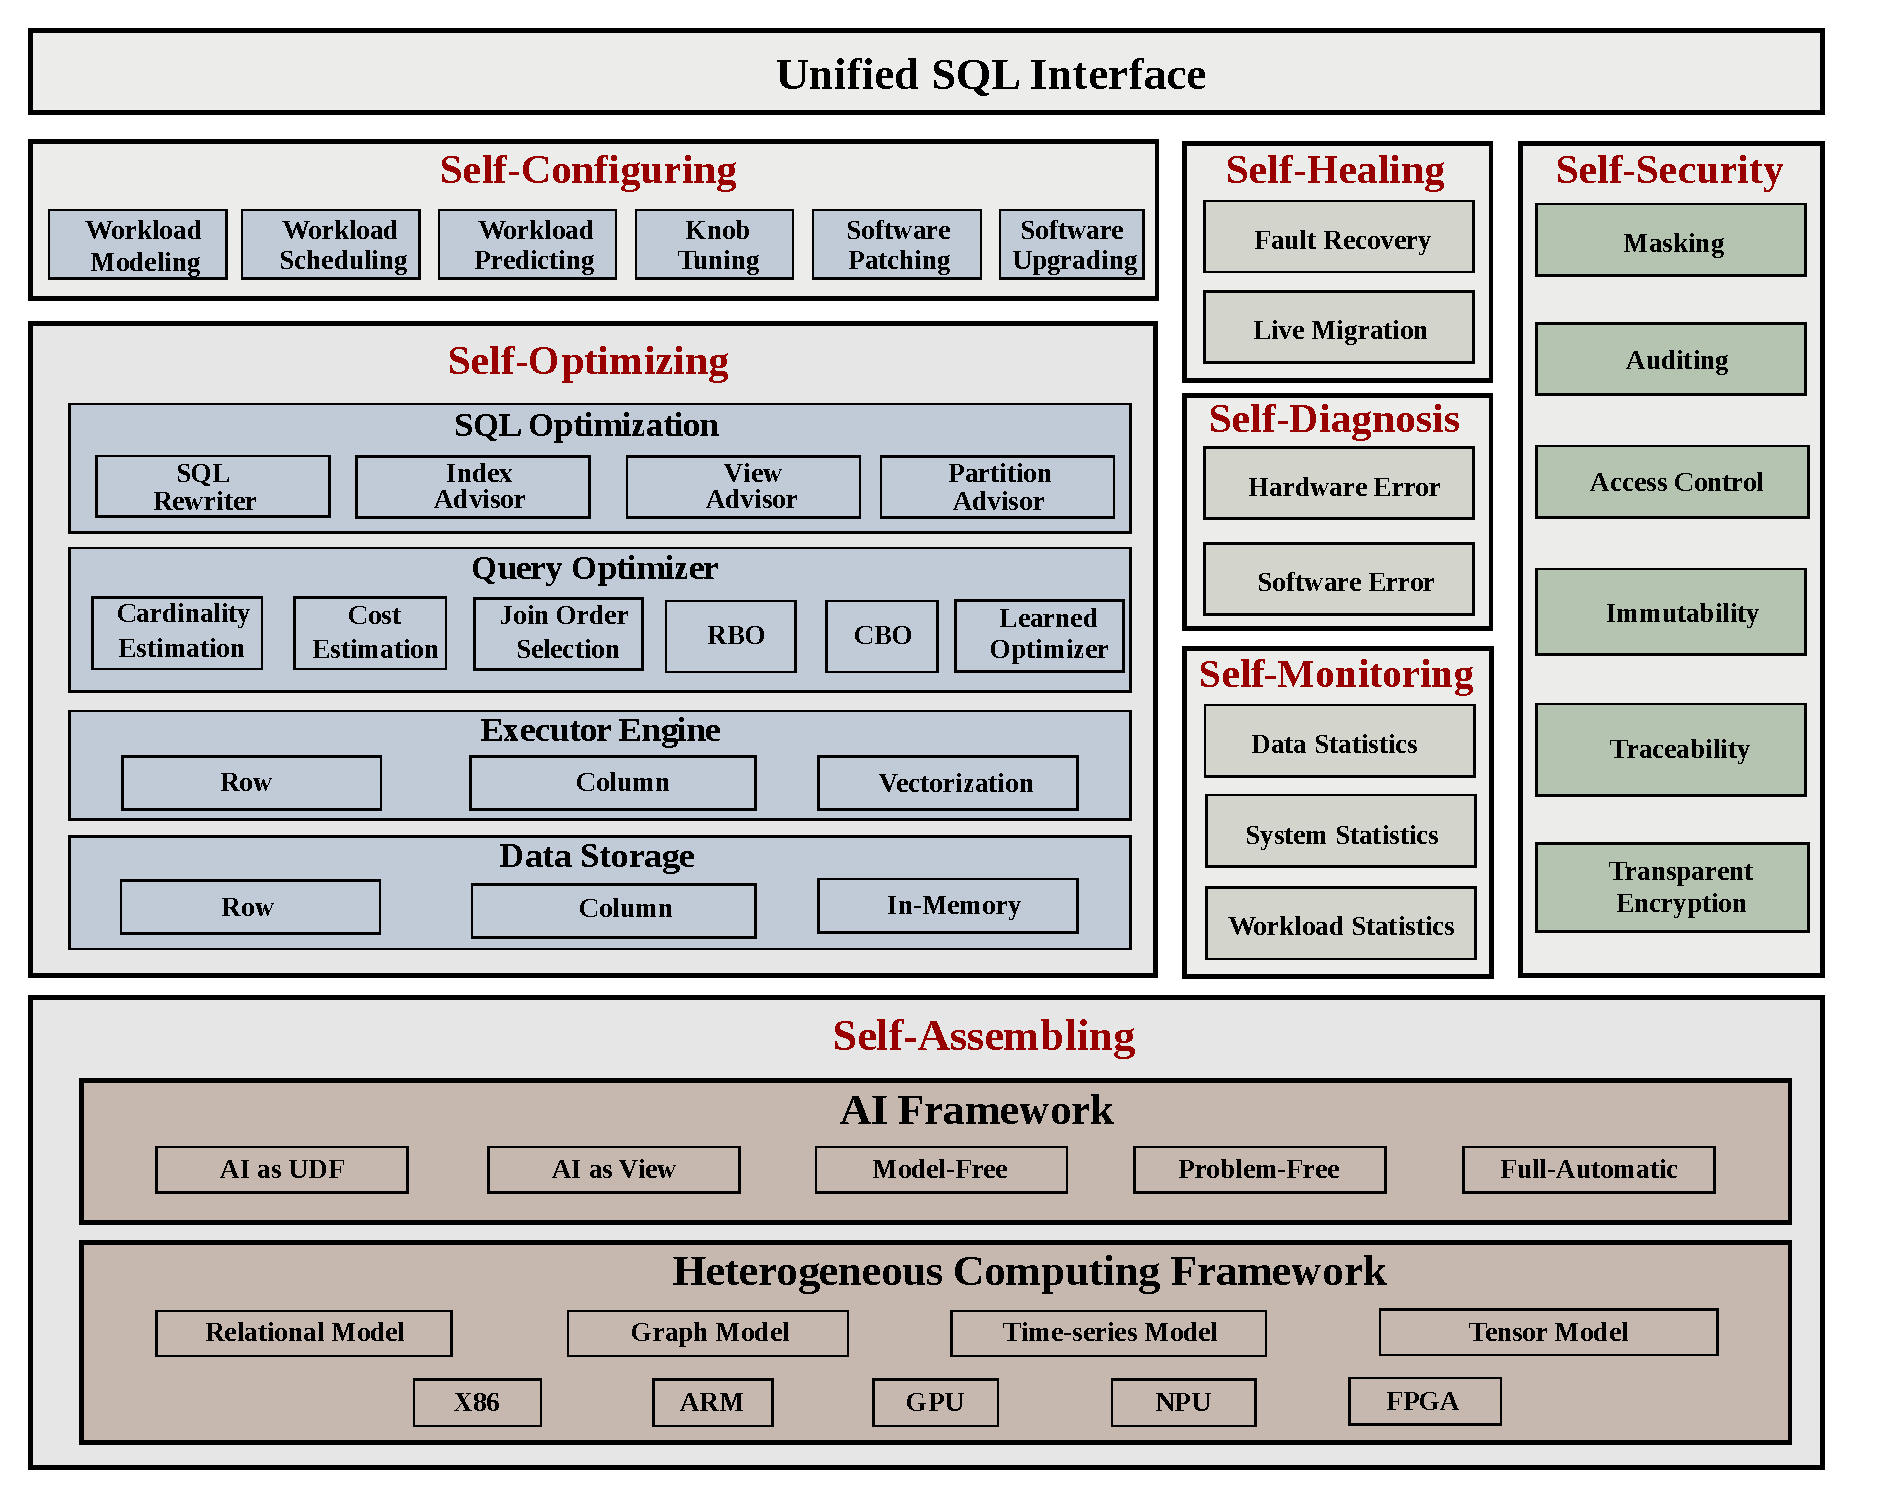
\includegraphics[width=1.0\textwidth, height=0.89\textwidth]{figs/ANDB-arch-v3.eps}
\vspace{-1em}
\caption{The architecture of AI-Native databases}
\label{fig:ANDB}
\vspace{-1em}
\end{figure*}

\begin{table}[!t]
\vspace{-1em}
\centering
\caption{Five levels of AI-native database}
\vspace{0.5em}

\label{tbl:ANDB}
{%\footnotesize
  \hspace*{-1em}
  \begin{tabular}{|c|c|l|l|}\hline
  
\multirow{1}{*}{\textbf{Level}} & \multirow{1}{*}{\textbf{Feature}} & \multirow{1}{*}{\textbf{\ \ \ \ \ \ \ \ \ \ \ \ Description}} & \multirow{1}{*}{\textbf{\ \ \ \ \ \ \ \ \ \ \ \ \ \ \ \ \ \ \ \ \ \ \ \ \ \ \ \ \ \ \ \ \ \ \ \ Example}} \\\hline

\multirow{4}{*}{\textbf{1}} & \multirow{4}{*}{AI-advised} & \multirow{4}{*}{Plug-in AI engine} &$\circ$ Workload Management (e.g., \small{workload scheduling})  \\
 &  & & $\circ$  SQL Optimization \small{(e.g., SQL rewriter, index/view advisor)} \\
 &  & &$\circ$  Database Monitor \small{(e.g., knob tuner, system statistics)}\\
 &  & &$\circ$  Database Security \small{(e.g., autonomous auditing/masking)}\\\hline

\multirow{6}{*}{\textbf{2}} & \multirow{6}{*}{AI-assisted} & \multirow{6}{*}{Built-in AI engine} &$\bullet$ Self-configuring (e.g., online knob tuning) \\
 &  & &$\bullet$ Self-optimizing (e.g., SQL optimization, data storage)\\
 &  & &$\bullet$ Self-healing (e.g., fault recovery, live migration)\\
 &  & &$\bullet$ Self-diagnosis (e.g., hardware/software error)\\
 &  & &$\bullet$ Self-monitoring (e.g., monitor workload/system state)\\
 &  & &$\bullet$ Self-security (e.g., tractable, encryption, anti-tamper)\\\hline

\multirow{7}{*}{\textbf{3}} & \multirow{7}{*}{AI-enhanced} & \multirow{7}{*}{Hybrid DB\&AI engine} &$\circ$ Learning-based Database Component \\
 &  & &\ \ \  $\bullet$ Learning-based rewriter\\
 &  & &\ \ \  $\bullet$ Learning-based cost estimator\\
 &  & &\ \ \  $\bullet$ Learning-based optimizer\\
 &  & &\ \ \  $\bullet$ Learning-based executor\\
 &  & &\ \ \  $\bullet$ Learning-based storage engine\\
  &  & &\ \ \  $\bullet$ Learning-based index\\
 &  & &$\circ$ Declarative AI (UDF; view; model-free; problem-free) \\\hline
\multirow{2}{*}{\textbf{4}} & \multirow{2}{*}{AI-assembled} & \multirow{2}{*}{Heterogeneous processing} & $\circ$ Self-assembling\\
&  & & $\circ$ Support new hardware (e.g., ARM, GPU, NPU)\\\hline

% &  &   &$\circ$  Extend relational algebra to support tensor model \\\hline

\multirow{1}{*}{\textbf{5}} & \multirow{1}{*}{AI-designed} & \multirow{1}{*}{The life cycle is AI-based} &Design, coding, evaluation, monitor, 
and maintenance \\\hline
  \end{tabular}
}
\vspace{-1em}
\end{table}


\hi{Workload Management}. AI-based models can be used to control the workload from three aspects. First, AI-based models can benefit workload modeling. Directly modeling a workload with independent features (e.g., tables, columns, predicates) may lead to great information loss, such as the reference correlations among different tables. So instead we use an encoder-decoder model to learn an abstract representation of user workloads, which can reflect the correlation among the basic features. Second, AI-based models can be used for workload scheduling. Considering hybrid OLAP and OLTP workloads, AI-based models can estimate the required resources (e.g., CPU, RAM, DISK) and running time of each query. Then AI-based models can prioritize the workload, assign a high priority for the mission-critical queries, and defer the execution of queries that require heavy resources. Moreover, resource scheduling depends heavily on some parameters related to resource control, e.g., maximum concurrent IO throughput. But these parameters are static and need to be manually configured. Reinforcement learning can be used to learn relations between database (physical/logical) states, workload and database resources, and provides a reasonable and robust scheduling mechanism. Third, AI-based models can be used for workload prediction. We can predict the possible workloads in order to adapt to future workloads. Traditional workload prediction methods rely on database experts based on statistical data, which can not guarantee high accuracy. Instead, machine learning methods for workload forecasting~\cite{DBLP:conf/sigmod/MaAHMPG18} have better adaptability to different workloads. 


%In order to avoid using CPU, IO and other system resources as workload metrics in different hardware environments, we use logical metrics to characterize workload, which further ensures the stability of prediction.

%estimate the It has two functions: to schedule user workloads and summary workload characters for the other modules. For \textsf{workload modeling}, traditional cost models are mostly based on empirical formulas, which have poor adaptability to different physical environments. Therefore, the machine learning model can be used to analyze and evaluate the current workload situation and future overhead, and dynamically adapt to the external environment based on gradient changes.
%For \textsf{workload scheduling}, in traditional databases, 
%For \textsf{workload predicting}, workload usually dose not change in a fixed pattern. 

\hi{SQL Optimization}. It optimizes SQL queries from the following aspects. First, {\it SQL rewriter} can rewrite the poor SQL queries issued by ordinary users into well-formulated queries in order to improve the performance. Traditional methods rely on DBAs, which are impractical for heavy workloads. So AI-based methods can provide a rewriting tool to learn the principles of SQL writing (e.g., avoiding full table scanning, selecting indexed columns for joins) and optimize the SQL structure. Second, {\it index advisor} can be optimized by AI-based methods. Database indexes are very important to improve the efficiency of SQL queries on complex data sets~\cite{DBLP:journals/kais/GaniSSH16}. However, the traditional methods build the indexes based on DBAs' experiences, which cannot scale to thousands of tables. AI-based models can learn the benefit and cost to build an index given a query workload, and then automatically recommend the index based on the learned information. Third, \textit{view advisor} can be optimized by AI-based models. Given a set of queries, we can first extract the equivalent sub-queries, select the sub-queries with high frequency, and learn the benefit and cost of building views on the sub-queries. Then materialized views can be automatically recommended by AI-based models. Fourth, {\it partition advisor} can be optimized by AI-based models. Traditionally the partitions are generated based on some primary keys or manually specified keys by DBAs. However, these methods may not find the best partition strategy. Instead, the AI-based models can learn the possible distribution of the partitions, estimate the benefits for different workloads, and recommend high-quality partitions.
 
%the commonly used indexes are universal data structures. They do not analyze and utilize the distribution of data. So through machine learning, we can learn a model that reflects data patterns, and can automatically synthesize a special index structure at a lower cost.
%, extracting high-frequency sub-queries and establishing materialized views to improve the performance of the database is very helpful. 
%The traditional method caches at the whole query level, and the hit rate is low.
%We construct the ML algorithm of sub-query selection according to the actual constraints so as to improve the query efficiency of batch SQL tasks.
%Generally speaking, it includes four kinds of methods: real-time monitoring, timing monitoring, analysis report, tracking and data collection. Performance monitoring is not only statistical indicators, but also needs to understand the operation of the system based on these indicators.  %It provides services (e.g., performance monitoring, tuning, fault tolerance) to ensure the stable operation of the database. In distributed scenario, high load pressure will lead to a sharp increase in failure rate, which brings great challenges to database maintenance. 

\hi{Database Monitor}. It monitors the database states, tunes database configuration and avoids database fail-overs. First, for \textit{data statistics}, it automatically monitors the access frequency on table columns, data updates, and data distribution among different shards.
Second, for \textit{system statistics}, it automatically monitors the status of the database system (e.g., the number of batch requests per second, the number of user connections, network transmission efficiency). Then it analyzes those indicators using machine learning algorithms, tunes system parameters and provides early warnings for abnormal events. Third, for \textit{workload statistics}, it monitors the performance of user workload and profiles on how workload varies. It can also predict  future workloads.

%states and tunes the states accordingly.
%Second, for \textit{database tuning}, database configuration involves hundreds of tunable system parameters, which control the database performances in many aspects. Traditional tuning methods~\cite{DBLP:journals/pvldb/DuanTB09, DBLP:conf/cloud/ZhuLGBMLSY17} either rely on DBAs, or cannot adapt to new workloads and environments. A deep-reinforcement-learning-based model~\cite{DBLP:conf/vldb/qtune19} can be used to learn relations between database state, query and parameters, which can adapt to environment changes dynamically. Third, for \textit{fault tolerance}, it includes a variety of strategies for resolving failures of hardware, transactions and systems. In case of failures, the system needs to terminate the corresponding transactions in time. An AI-based model can be used to monitor the changes caused by typical failures and provides early warning. 

%Existing masking techniques only uses the high-dimensional, non-linear data inside the neural network to help improve the effect of data hiding. For example, in the research project conducted by Stanford University and Google, satellite images have been converted into high-frequency signals that are not easily detected.

\hi{DB Security}. It combines security and cryptography technology with AI techniques to enhance the security of databases. First, \textit{autonomous masking} aims to hide privacy data such as ID number. Autonomous masking judiciously selects which columns to be masked based on historical data and user-access patterns. Second, \textit{autonomous auditing} optimizes the auditing from two aspects: data pre-processing and dynamic analysis. Traditional auditing often requires auditors to obtain a large number of business data, which is hard to obtain. Autonomous auditing not only saves manpower cost, but also helps auditors to make better decisions by providing useful information from massive data.  Third, \textit{autonomous access control} can automatically detect system vulnerabilities. Existing autonomous detecting methods are mainly to retrieve through security scanning, but cannot detect unknown security vulnerabilities.  AI-based models can discover security vulnerabilities~\cite{DBLP:journals/corr/abs-1902-10680}, which not only detect the most known vulnerabilities in a vulnerability database, but also predict and evaluate potential vulnerabilities.  


\subsection{Level 2: AI-Assisted Database}
\label{subsec: assisted}

The second level, AI-assisted databases, integrates an AI engine into the database kernel for run-time optimization. AI components (e.g., tuning model, workload scheduling, view advisor) can be merged into the corresponding database components~\cite{DBLP:journals/corr/abs-1903-01363}. In this way, AI capabilities are integrated into the working procedure of the database. For example, if embedding the tuning model into the query optimizer, we can first conduct query tuning for each query (e.g., tuning user-level parameters to better adapt to the query features), and then normally generate and execute the query plan. The advantage of AI-assisted databases is that 1) it can provide more fine-grained optimization; 2) it can reduce more overhead by embedding an AI engine into the kernel. 

%However, neither Level 1 or 2 is a real AI-native database. Because the main components and organizing mode in those databases are still based on traditional methods. There are huge gap between AI technologies and databases. Starting from the third level, we introduce how to integrate intelligence integration, heterogeneity into database design to achieve the AI-native database.

Moreover, built-in AI engine can provide self-configuring, self-optimizing, self-monitoring, self-healing, self-diagnosis, and self-security services. 

\hi{Self-configuring}. Database can automatically tune their own configuration to adapt to changes in workload and environment. First, the workload can be  self-configured. Database can execute queries in different granularities in parallel, each of which has various requirement of system resources and performance. Database can configure the workload based on the workload features, which are obtained by conducting workload modeling, scheduling and predicting. Second, databases include several configuration mechanisms, such as knob tuning, software patching, software upgrading and etc. For example, all databases have hundreds of tuning knobs, which are vital to nearly every aspect of database maintenance, such as performance, availability, robustness, etc. However, these configurations require to be tuned manually, which not only is time consuming but also cannot find optimal configurations. AI based methods, e.g., deep reinforcement learning, can automatically tune the database knobs. Moreover, other configurations (e.g., software bugs, partition scheme) can also be optimized by AI-based methods. 

%Each function is embedded into particular DB modules to work as part of the processing.  For example, to realize tuning in query level, we embed tuner into optimizer. Each time a parse tree is input into our optimizer, it first configures parameters based on the query features and then actually generates the query plan. This way, it not only helps to generate better query plan, but prepares suitable environment for executing the query plan. 
%We achieve self-optimizing by designing learning-based query optimizer and hybrid executing and storing components.  


\hi{Self-optimizing}. 
First, we can design a learning-based query optimizer in cost/cardinality estimation, join order selection and data structures. 1) AI techniques can optimize cost/cardinality estimation, which is vital to query plan selection. However, database mainly estimates cardinality based on raw statistics (e.g., number of distinct values, histograms)  and is poor in estimating the resulting row number of each query operator (e.g., hash join, aggregate, filter), by using histograms. AI-based methods, e.g., Tree-LSTM, can learn data distribution in depth and provide more accurate cost/cardinality estimation. 2) AI techniques can optimize join order selection. Different join schemes have a great impact on query performance and finding the best plan is an NP-hard problem. With static algorithms (e.g., dynamic programming, heuristics algorithm), the performance of join order selection in databases is limited by the quality of the estimator. AI-based methods can better choose between different join order plans by taking one-step join as the short-term reward and the execution time as the long-term reward. 3) Data partitions, indexes, and views can also be online recommended by built-in AI models.  
Second, we can utilize learning-based models to optimize executor engine and data storage. For executor engine, we consider two aspects. 1) We provide hybrid query executing methods such as row-based and column-based. Here AI can serve different data applications (e.g., row-based for OLTP, column-based for OLAP). 2) We provide tensor processing engine to execute AI models. To enhance AI techniques to optimize database components, databases can execute AI models natively with a vectorization engine. % Similarly, we design data storage from two aspects. 1) Data storage for AI models (e.g., training data, trained AI models) and database (e.g., user data, database statistics) based on the data characters. 2) In-memory data storage. By buffering AI models and hot data in memory, we can enhance database service quality.

%Database can automatically collect statistics of queries and optimize database performance in multiple granularities. Firstly, it collect statistics used in optimizer to learn current workload, which can benefit from cardinality estimation and workload scheduling. Secondly, it automatically design index, materialized query table (MQT) and data partition, which can directly optimize performance of single query. Thirdly, it automatically controls the flow of queries with query patroller to achieve overall optimization.


\hi{Self-monitoring}. Database can automatically monitor database states (e.g., read/write blocks, concurrency state, working transactions) and detect operation rules, e.g., root cause analysis rules. It can monitor database states (e.g., data consistency, DB health) in the life-cycle. The monitored information can be used by self-configuring, self-optimizing, self-diagnosis, and self-healing. Note that it may have some overhead to monitor the database states and we need to minimize the overhead for monitoring database states. %And by concluding all the fail-over conditions and solutions, it can translate the experience in the form of publication of instrumentation data in favor of human understanding.


%For example, rather than cleaning dirty pages in memory every fixed time, we replace the timing part  with the results of workload forcasting, which can predict how the workload varies. And it conducts cleaning when DB is free.live migration, checkpoint,  logging each write operations, we can focus on recording 

\hi{Self-diagnosis}. Self-diagnosis includes a set of strategies to diagnose and correct abnormal conditions in databases, which are mostly caused by errors in hardware (e.g., I/O error, CPU error) and software (e.g., bugs, exceptions). Self-diagnosis helps to guarantee services even if some database nodes work unexpectedly. For example, in case of data-access error, memory overflow or violation of some integrity restrictions, database can automatically detect the root causes using the monitored states and thus cancel the corresponding transactions in time. 


%Database can automatically monitor processing procedure of each query and prevent potential damage in time. For example, it can throttle service requests which compete resources to cut down deadlock and average waiting time; and it can kill or lower the priority of run-away queries (execution time is far longer than that estimated by the optimizer) to prevent from using up system resources. Besides, database can guarantee the security of each session by detecting potential security vulnerabilities and masking sensitive data from available. \lgl{}




\hi{Self-healing}. Databases can automatically detect and recover from database problems (e.g., poor performance, hardware/software fail-overs). First, it isolates different sessions or users and avoids affecting others users when encountering errors. Second, it adopts AI-advised database tools to reduce the recovery time and saves humans from the failure-recovery loop. Third, it can kill some abnormal queries that take too many resources. 
%For example, 
%First, it predicts possible problems (e.g., backup, data sharding, resource scheduling) and is robust to system faults (e.g., cope with incorrect input). Second, it can maintain services even if emergency occurs (e.g., live migration).


\hi{Self-security}. Self-security includes several features. First, the data in the life-cycle (including storage, memory and CPU) are always encrypted, which should be unreadable for the third party. Second, the data access records should be tractable in order to get the access  history of the data. Third, the data should be tamper-proofed in order to prevent malicious modification of data. Fourth, AI-based models can be used to automatically learn the attacking rules and prevent the unauthorized access and attack patterns. Fifth, it can automatically detect sensitive data using AI-based models. 

%  1) Immutable. To protect database from tampering externally. 2) Tractable. Any data access can be recorded in time series. 3) Transparent encryption. With AI-based methods, it performs encryption and decryption of database data and log in real-time I/O. Besides, it can help decide proper encryption algorithms for different data without altering applications and achieve this in real-time.

\subsection{Level 3: AI-Enhanced Database}
\label{subsec: enhanced}

The third level, AI-enhanced database, not only uses AI techniques to improve the database design but also provides in-database AI capabilities. 

%intelligence and integration into database design. 
%Firstly, we propose an intelligent database kernel, which implants AI into the design of database kernel. Secondly, we propose a  unified engine for both AI and DB, with which clients can use AI as easily as they use a DB.

\subsubsection{Learning-based Database Components}
\label{subsubsec: intelligent}

Most of database core components are designed by humans based on their experiences, e.g., optimizer, cost estimation, index. However, we find that many components can be designed by AI-based models. First, the traditional indexes, e.g., B-tree, R-tree, can be designed by AI-based models. For example, learned indexes are verified that they can reduce the index size and improve the query  performance~\cite{DBLP:conf/sigmod/KraskaBCDP18}. Second, the cost/cardinality estimation can be optimized by deep learning, because the empirical methods cannot capture the correlations among different tables/columns while deep learning can capture more information using deep neural networks. Third, the join order selection problem is an NP-hard problem and traditional heuristics methods cannot find the best plan; while the deep reinforcement learning techniques can learn more information and get better plan. Fourth, query optimizer replies on cost/cardinality estimation, indexes, join order selection, etc, and an end-to-end learning based optimizer is also promising. 

Thus many database components can be enhanced by AI-based methods, which can provide alternative strategies beyond traditional empirical techniques. 

%We present the design of an intelligent database kernel that enables self-configuring, self-healing, self-optimizing, self-protecting, self-inspecting and finally achieves self-organizing.


\subsubsection{In-Database AI Capabilities}
\label{subsubsec: engine}

Although AI can address many real-world problems, there is no widely deployed AI systems that can be used in many different fields, because AI is hard to be used by ordinary users. Thus we can borrow database techniques to lower the barrier of using AI.  First, SQL is easy to be used and widely accepted, and we can also extend SQL to support AI. Second, we can utilize database optimization techniques to accelerate AI algorithms, e.g., indexing, incremental computing, and sharing computations. 


We categorize the techniques of supporting AI capabilities in database in five levels. 

% as shown in \lgl{Table~\ref{tbl:AI}}.
%shows, Database supports AI services in five levels.
%Presently, DB mainly serves for structured data analysis such as financial transactions. By embedding AI algorithms into DB engine, DB can directly support many AI applications (e.g., image comparison, graph computing) in an end-to-end way. As Figure~\ref{fig:DB4AI} shows,  

\hi{AI Models As UDFs}. We embed AI frameworks (e.g., MADlib, TensorFlow, Scikit-learn) in database and provide user-defined functions (UDFs) or stored procedures (SPs) for each algorithm. Then users can call UDFs or SPs from databases to use AI algorithms. 

\hi{AI Models As Views}. If a user wants to use AI algorithms (e.g., random forests) in the first level, the user requires to first train the model and then use the trained model. In the second level, we can take an AI algorithm as a view, which is shared by multiple users. If an algorithm is used by a user, we can materialize the model and other users can directly use the model. The model can also be updated by incrementally training. 

%is updatedDatabase provides classic AI models . Clients can directly call AI models from database and only focus on the training part. 

%$\bullet$ \textbf{DB-based AI Process}. Database further provides AI processes, which not only include the mature AI models but the training methods (e.g., SGD, Adam, reinforcement learning). Clients can directly call AI processes from database, only with data as input. Database automatically fine-tunes AI model using corresponding training method, and utilizes the model to produce results. 

\hi{Model-free AI}. In the first and second levels, the user must specify the concert algorithms (e.g., k-means for clustering). Actually, users may only know which problems should be addressed, e.g., clustering or classification, but do not know which algorithms should be used. In this way, database can automatically recommend the algorithms that best fit the user scenarios.

%Database can automatically parse the requirements in AI and call proper process to solve it. Clients only need to declare their requirement. For example, if we hope to search some images, we just declare the conditions and data sources with SQL. And database automatically chooses the CNN model to conduct the work, which is also a part of the query plan.

\hi{Problem-free AI}. The users even cannot specify the problems that require to be addressed, e.g., classification and clustering. Given the database, the problem-free AI can automatically find which problems can be addressed by AI algorithms and recommend suitable AI algorithms. 

\hi{Full-automatic}. The system can automatically discover AI opportunities, including discovering the problems, the models, the algorithms, relevant data,  and training methods.  

%The users even cannot specify the problems that require to be addressed. Given the data, the problem-free AI can automatically find which problem can be addressed by AI algorithms and recommend the best AI algorithms.

% Database offers an insight into the data schema and application queries, and optimizes itself with AI techniques. For example, if a new workload comes, database can call a DRL-based tuner to adjust the system parameters based on the query features, including cost estimation, resource allocation, concurrency  control and etc. 

\iffalse
\begin{table}[!t]
\vspace{-1em}
\centering
\caption{Five levels of machine learning consumability in DBMS}
\label{tbl:AI}
{%\footnotesize
  \hspace*{-0em} \begin{tabular}{|c|c|l|c|c|}\hline
  
\multirow{2}{*}{\textbf{Level}} & \multirow{2}{*}{\textbf{Consumability}} & \multirow{2}{*}{\textbf{\ \ \ \ \ \ \ \ \ \ \ \ \ \ \ \ \ \ \ \ \ \ \ \ Description}} & \multirow{2}{*}{\textbf{Target Users}} & $\textbf{ML Skill}$ \\
 &  &  & & $\textbf{Level}$ \\\hline

\multirow{2}{*}{\textbf{1}} & \multirow{2}{*}{Algorithm} & \multirow{2}{*}{Algorithms as UDFs and stored procedures} & Data scientists,  & \multirow{2}{*}{High} \\
 &  & & experienced developers & \\\hline


\multirow{2}{*}{\textbf{2}} & \multirow{2}{*}{Model} & Models as first-class object with DDL, & App. developers  & \multirow{2}{*}{Medium} \\
 &  &  DCL, DML capability  & and DBAs & \\\hline

\multirow{2}{*}{\textbf{3}} & \multirow{2}{*}{Process} &  Processes as first-class object with DDL, & App. developers & \multirow{2}{*}{Low} \\
 &  & with DCL, DML capability  & and DBAs & \\\hline

\multirow{2}{*}{\textbf{4}} & \multirow{2}{*}{Automation} &  Problem specifications as first-calss object & Business specialists, DBAs & \multirow{2}{*}{Low} \\
 &  & with DDL, DCL, DML capability  & app. developers & \\\hline


\multirow{2}{*}{\textbf{5}} & \multirow{2}{*}{Discovery} &  Discover ML opportunities based on & Business specialists, DBAs & \multirow{2}{*}{Very Low} \\
 &  & data schema and application queries  & app. developers & \\\hline

  
  \end{tabular}
}
\vspace{-1em}
\end{table}
\fi

\subsubsection{Hybrid AI and DB Engine}
\label{subsubsec: engine}

The above methods still use two engines: AI engine and DB engine. It calls for a hybrid AI and DB engine that provides both AI and DB functionalities. Then given a query, the SQL parser parses the SQL query and produces a general-purpose query plan. Based on the operators in the plan, it decides whether it utilizes relational data models or utilizes AI models. For relational data models, the query plan is sent to the database executor; otherwise, it is sent to the AI executor. Moreover, it also calls for new models to support both relational algebra and tensor models, and in this way, we can utilize a unified model to support both AI and database. 

%We extend the relational algebra theory to support both relational and tensor data models. 




%This way, DB can support tensor processing, which is largely used in the training of AI models.


%After achieving the intelligent database kernel, we gain real integration by providing unified engine for DB and AI. AI and DB are closely connected. For DB, as talked above, AI can make DB  smarter. For AI, DB stores large scale of data for training the ML models. 
%So it becomes easy when we can call ML model with SQL statements. 

%For this work, there have been some products such as BigQuery ML~\cite{DBLP:conf/ideas/FernandesB15}, SQL for DL and SQLFlow. Considering the Pros and Cons of these works, we propose an extended DB engine to achieve the following aims:

%$\circ$ \textbf{AI Support}. Firstly, SQL Parser should extend SQL syntax to utilize AI methods, including model creating, training and predicting. Besides, it should minimize the use of other scripting languages (e.g., Python and R). Secondly, 


%$\circ$ \textbf{General Purpose}. SQL parser should contain an abstract layer which maintains a loose couple with lower components. This way, it can be easily used on different SQL engines (e.g., PostgreSQL, Flink and Hive) or machine learning toolkits (e.g., TensorFlow, Keras and scikit-learn). 

%$\circ$ \textbf{Custom Style}. Besides general operators such as SELECT and WITH, we also allow user to define how to train, evaluate and predict the ML models with user-defined functions. And they also can cache the trained model with materialized views.


%This way, database can also provide AI services in an end-to-end way. 

%\begin{figure}[!t]%{0.5\textwidth}
%\centering
%\includegraphics[width=0.48\textwidth,height=0.3\textwidth]{figs/assembing.eps}
%\vspace{-1em}
%\caption{AI-Assembled Database}
%\label{fig:assemble}
%\vspace{-1em}
%\end{figure}

\subsection{Level 4: AI-Assembled Database}
\label{subsec: assemble}

The fourth level, AI-assembled database, not only automatically assembles database components to generate a database that can best fit a given scenario, but also schedules the tasks to diversified hardware. 



\hi{Self-assembling}. First, each database component has multiple options. For example, optimizers include cost-based model, rule-based model, and learned-based model. We first take each component variant as a service. Then we select the best components based on users' requirements. Note that different variants of the same component should adopt the same standard interface such that the components can be assembled. 

\begin{wrapfigure}{r}{0.55\textwidth}
\vspace{-2em}
  \begin{center}
    \includegraphics[width=0.6\textwidth,height=0.35\textwidth]{figs/assembing.eps}
  \end{center}
\vspace{-3em}
\caption{AI-Assembled Database}
\label{fig:assemble}
\vspace{-1em}
\end{wrapfigure}


%has multiple standardized components to choose from. How to choose the appropriate processing path for one or a batch of queries becomes meaningful. 

Thus we propose a self-assembling module. For different scenarios, we can dynamically select the appropriate components in each layer of service and assemble the appropriate execution path. The execution path can be seen as a natural language sequence (NLS), such as $\langle$ $SQL_i$, parser$\_$pg, optimizer$\_$RBO, storage row, accelerator $\rangle$, in which each position has only discrete token options. So the problem is how to generate NLS in the query level. One possible method is to use reinforcement learning (RL)  algorithm. It takes the whole path sequence as an episode and a single action as an epoch. Under each epoch, the agent chooses the next component (action), which executes the query, leading to a state transition (e.g., the query status changes into syntax tree). In this problem, action is discrete, so DDQN algorithm~\cite{DBLP:conf/aaai/HasseltGS16} can be used. Compared with other RL algorithms with discrete outputs,  DDQN eliminates the problem of overestimation (deviate greatly from the optimal solution) by choosing decoupling actions and calculating the target Q value.


However, the RL-based routing algorithm has two problems.  Firstly, Q network will not generate scores until the last node is generated. It is insensitive to the choice of intermediate nodes. However, for the entire path, it is necessary to give an action a comprehensive score on current and future impacts. 
Secondly, when training with epoch as a unit, each node of a path is scattered in a training sample, instead of being used as a whole to calculate the gradient. 


Generative Adversarial Network (GAN)~\cite{DBLP:journals/corr/abs-1902-05687} can better solve those problems of end-to-end path selection. We use G network to generate path vectors based on the workload, database state and component characteristics, and we use D network as the performance model. 
But the traditional GAN network model is not fully applicable to our problem. Because it is mainly used to generate data with continuous range of values, and it is difficult to generate path vectors with discrete tokens. That is because G-networks need to be fine-tuned based on gradient descent and regress towards the expectation. But when the data is discrete tokens, fine-tuning is often meaningless. So we choose to combine RL algorithm with GAN~\cite{DBLP:conf/aaai/YuZWY17}. Firstly, G network is used as an agent in the RL algorithm: action is the next service node; state includes not only query status, database status, but also generated node information. Each iteration generates a complete path. Secondly, unlike the traditional RL algorithm, each action is scored by D network to guide the generation of the whole path sequence.

\hi{Heterogeneous Computing.} We need to make full use of diversified computing power. Note that DB and AI usually require different computing power and hardware. For DB, traditional optimizer processes queries with CPU. While AI requires new AI chips to support parallel processing (e.g., GPU and NPU) and self-scheduling. And now many applications need to use both DB and AI techniques, especially in large data analysis scenarios.  Thus we need to support multiple models, e.g., relation model, graph model, stream model and tensor model. We can automatically select which models should be used. We also need to be able to switch computing powers based on the models. For example, for the tuning module in the optimizer, when training the tuning model, we fetch training data into memory with AI chips and conduct backward propagation (training the neural network) with NPU. For the join and selection operations, we may still use the traditional hardware. We also need to study whether a model (e.g., relational model) can be transformed into other models (e.g., tensor model).  The ultimate objective is to fully unleash the power of diversified computing, including x86, ARM, GPU, NPU. We aim to continuously push our AI strategy forward and foster a complete computing ecosystem. 


%It can utilize different computing powers to better serve the AI components. 
%And database should flexibly schedule computing powers, e.g., when NPUs are overburdened but most ARM resources are idle, ARM array can share some burden.

%AI-assembled database mainly has two contributions. Firstly, it can support ARM architecture. 
%1) It effectively utilizes ARM array with multi-core mode, inter-node parallelism, intra-node parallelism, instruction-level parallelism, compiler parallelism and other super-parallel technologies. 
%2) For the problem of competition brought by multi-core, it provides cross-chip access optimization and resource scheduling optimization. 

%Secondly, 



\subsection{Level 5: AI-Designed Database}
\label{subsec: designed}

The fifth level, AI-designed databases, is fully designed by AI, including design, coding, evaluation, monitoring and maintenance. In this way, AI techniques are integrated into the whole database life cycle so as to achieve the best performance for both DB and AI.

%ultimate goal that (1) the database  scenario-aware and AI-as-a-service. 














%The whole life cycle includes five phases: 1) Database initialization; 2) Database design; 3) Database implementation; 4) Database evaluation; 5) Database operation and maintenance.


%To alleviate the issues talked above, in this section we propose a design of AI-native database, which better provides DB and AI services in five levels. 




